\documentclass[../Cover.tex]{subfiles}

\begin{document}
	\begin{minipage}[t][0.2\textheight][t]{0.1\textwidth} 
		
\includegraphics[width=\textwidth]{DC.png}
	\end{minipage}
	\hfill
	\begin{minipage}[t][0.2\textheight][t]{0.8\textwidth}
		\begin{tabular}{ p{0.25\textwidth} l  }			
			\\
			\small \textbf{Changing Gears Drill} \\
			\\[0.09\textheight]
		\end{tabular}
		\quad
		%%%%%%%%%%%%%%%%%%%%%%%%%%%
		% Quick Facts Table       %
		%%%%%%%%%%%%%%%%%%%%%%%%%%%
		\begin{tabular}{ | p{0.2\textwidth} | p{0.2\textwidth} | p{0.1\textwidth} |}
			\hline
			\rowcolor[HTML]{C0C0C0}\tiny Weapon Type & \tiny Distance & \tiny Par Time\\ 
			\hline
			\tiny Pistol & \tiny 7yd & \tiny 4s \\ % EDIT HERE
			\hline
		\end{tabular}
	\end{minipage}
	%%%%%%%%%%%%%%%%%%%%%%%%%%%
	% Requirements      %
	%%%%%%%%%%%%%%%%%%%%%%%%%%%
	\begin{tabular}{p{0.25\textwidth}}
		\small Requirements \\
		\hline
		\tiny \begin{itemize} % EDIT HERE
			\item Two targets, one 8" circle, one 3x5" card.
			\item Rounds fired: 4+
			\item Starting Position: Holstered 
		\end{itemize}		
		\begin{center}
			

\tikzset{every picture/.style={line width=0.75pt}} %set default line width to 0.75pt        

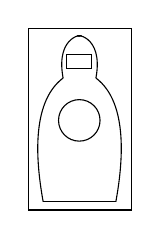
\begin{tikzpicture}[x=0.75pt,y=0.75pt,yscale=-0.4,xscale=0.4]
%uncomment if require: \path (0,300); %set diagram left start at 0, and has height of 300

%Curve Lines [id:da6503959532228425] 
\draw    (310.5,95) .. controls (300.5,41) and (339.5,42) .. (330,45) ;


%Curve Lines [id:da36557258563164563] 
\draw    (286.5,244) .. controls (278.5,200) and (270.5,125) .. (310.5,95) ;


%Curve Lines [id:da4587631559171017] 
\draw    (350.04,95) .. controls (360.04,41) and (320.5,42) .. (330,45) ;


%Curve Lines [id:da3685102327196659] 
\draw    (374.04,244) .. controls (382.04,200) and (390.04,125) .. (350.04,95) ;


%Straight Lines [id:da02283089550847861] 
\draw    (374.04,244) -- (286.5,244) ;


%Shape: Circle [id:dp5367594803674913] 
\draw   (305,146) .. controls (305,132.19) and (316.19,121) .. (330,121) .. controls (343.81,121) and (355,132.19) .. (355,146) .. controls (355,159.81) and (343.81,171) .. (330,171) .. controls (316.19,171) and (305,159.81) .. (305,146) -- cycle ;
%Shape: Rectangle [id:dp6278308195846618] 
\draw   (315,67) -- (345,67) -- (345,83) -- (315,83) -- cycle ;
%Shape: Rectangle [id:dp27764233136797056] 
\draw   (268.5,35) -- (392.5,35) -- (392.5,254) -- (268.5,254) -- cycle ;




\end{tikzpicture}
	
		\end{center}
		\\[0.6\textheight]
	\end{tabular}
	% Steps and Scoring	
	\begin{tabular}{ | p{0.65\textwidth} |}
		\hline
		%%%%%%%%%%%%%%%%%%%%%%%%%%%
		% Steps                   %
		%%%%%%%%%%%%%%%%%%%%%%%%%%%
		\rowcolor[HTML]{C0C0C0}Steps\\ 
		\hline
		\tiny \begin{enumerate}[topsep=0pt, partopsep=0pt]
			\item Slow-Fast: Draw, fire two rounds at the 3x5" card, then as many rounds as you can on the 8" circle before par time.
			\item Fast-Slow: Draw, fire two rounds at the 8" circle, then as many rounds as you can on the 3x5" card before par time.
		\end{enumerate}		
		\\ [0.25\textheight]
		\hline
		%%%%%%%%%%%%%%%%%%%%%%%%%%%
		% Scoring                 %
		%%%%%%%%%%%%%%%%%%%%%%%%%%%
		\rowcolor[HTML]{C0C0C0}Scoring \\
		\hline
		\tiny \begin{itemize}[topsep=0pt, partopsep=0pt]
			\item The goal of this drill is to practice switching between fast fire and precision, in both directions.
			\item The Small target is worth 10pts.
			\item The Large target is worth 5 pts.
			\item for added challenge, reduce the par time once you can land 5-6 rounds per run.
			\item Passing Hit Factor HF): 10.0
		\end{itemize}		
		\\ [0.25\textheight]
		\hline
	\end{tabular}
\end{document}
